\documentclass[12pt, a4paper, oneside]{report}

% Pachete esențiale
\usepackage[utf8]{inputenc}
\usepackage[romanian]{babel}
\usepackage[margin=2.5cm]{geometry}
\usepackage{graphicx}
\usepackage{amsmath}
\usepackage{booktabs}
\usepackage{setspace}
\usepackage{color}
\usepackage{listings}
\usepackage[hidelinks]{hyperref}

% Setări de spațiere
\onehalfspacing

% Stil pentru cod (Matlab)
\definecolor{codegreen}{rgb}{0,0.6,0}
\definecolor{codegray}{rgb}{0.5,0.5,0.5}
\definecolor{codepurple}{rgb}{0.58,0,0.82}
\lstdefinestyle{mystyle}{
    language=Matlab,
    commentstyle=\color{codegreen},
    keywordstyle=\color{blue},
    numberstyle=\tiny\color{codegray},
    stringstyle=\color{codepurple},
    basicstyle=\ttfamily\scriptsize,
    breaklines=true,
    captionpos=b,
    numbers=left,
    numbersep=5pt,
    tabsize=2
}
\lstset{style=mystyle}

\begin{document}

% --- PAGINA DE TITLU MANUALA ---
\begin{titlepage}
    \centering
    \vspace*{1cm}
    {\large UNIVERSITATEA NAȚIONALĂ DE ȘTIINȚĂ ȘI TEHNOLOGIE \\ POLITEHNICA BUCUREȘTI}\\[0.5cm]
    {\large FACULTATEA DE ELECTRONICĂ, TELECOMUNICAȚII ȘI \\ TEHNOLOGIA INFORMAȚIEI}\\[2cm]
    
    {\Large \textbf{LUCRARE DE DIZERTAȚIE}}\\[1.5cm]
    
    {\huge \textbf{Amplificator audio multicanal cu procesor digital de semnal programabil}}\\[2cm]
    
    \vfill
    
    \begin{flushleft}
        \large \textbf{Conducător științific:}\\
        Ș.L. dr. ing. Victor POPA
    \end{flushleft}
    
    \begin{flushright}
        \large \textbf{Absolvent:}\\
        Zglimbea Andrei
    \end{flushright}
    
    \vfill
    
    {\large BUCUREȘTI\\ 2026}
\end{titlepage}

% --- FRONT MATTER ---
\pagenumbering{roman}
\tableofcontents
\listoffigures

\chapter*{Lista acronimelor}
\addcontentsline{toc}{chapter}{Lista acronimelor}
\begin{description}
    \item[DSP] Digital Signal Processor
    \item[ADC] Analog-to-Digital Converter
    \item[DAC] Digital-to-Analog Converter
    \item[CMRR] Common Mode Rejection Ratio
    \item[SNR] Signal-to-Noise Ratio
    \item[THD] Total Harmonic Distortion
    \item[I2C] Inter-Integrated Circuit
\end{description}

\clearpage
\pagenumbering{arabic}

% --- CAPITOLE ---
\chapter*{Introducere}
\addcontentsline{toc}{chapter}{Introducere}

\section*{Motivație}
\addcontentsline{toc}{section}{Motivație}

În contextul actual al tehnologiei audio, flexibilitatea și calitatea procesării semnalului au devenit cerințe fundamentale atât în mediul profesional, cât și în cel de larg consum. Trecerea de la procesarea pur analogică la cea digitală a deschis noi oportunități pentru optimizarea răspunsului în frecvență, corecția acustică a spațiilor și implementarea unor algoritmi complexi de filtrare și dinamică.

Motivația acestui proiect rezidă în necesitatea de a crea un sistem audio versatil care să combine performanța etajelor analogice de precizie cu puterea de calcul a unui procesor digital de semnal (DSP). Un astfel de sistem permite utilizatorului să adapteze comportamentul amplificatorului în timp real, oferind o soluție compactă și eficientă pentru aplicații multimedia avansate.

\section*{Obiective}
\addcontentsline{toc}{section}{Obiective}

Obiectivul principal al lucrării este proiectarea, simularea și implementarea practică a unui amplificator audio multicanal dotat cu un procesor digital de semnal programabil. Pentru atingerea acestui scop, au fost stabilite următoarele obiective secundare:
\begin{itemize}
    \item Proiectarea unor interfețe de intrare compatibile cu standardele profesionale (+4dBu) și consumer (-10dBV), utilizând circuite balansate și nebalansate.
    \item Implementarea unui etaj de preamplificare cu zgomot redus bazat pe amplificatoare operaționale SoundPlus\texttrademark.
    \item Integrarea procesorului de semnal ADAU1701 și configurarea acestuia pentru procesare în timp real la 48kHz.
    \item Realizarea unui sistem de alimentare eficient, capabil să susțină atât etajele analogice de mic semnal, cât și etajele de putere în Clasa D.
    \item Dezvoltarea unui programator USB pentru configurarea facilă a algoritmilor DSP prin interfața SigmaStudio.
    \item Validarea performanțelor sistemului prin simulări software și măsurători experimentale.
\end{itemize}

\section*{Aplicabilitate}
\addcontentsline{toc}{section}{Aplicabilitate}

Sistemul propus își găsește aplicabilitatea în diverse domenii ale ingineriei audio și producției multimedia:
\begin{enumerate}
    \item \textbf{Sisteme de monitorizare audio:} Permite calibrarea precisă a boxelor de monitorizare în funcție de acustica camerei.
    \item \textbf{Prototipare rapidă:} Utilizarea DSP-ului programabil facilitează testarea rapidă a unor noi algoritmi de crossover, egalizare sau compresie fără modificarea hardware-ului.
    \item \textbf{Instalații audio personalizate:} Flexibilitatea intrărilor și ieșirilor face sistemul ideal pentru instalații fixe în spații comerciale sau rezidențiale unde este necesară o gestionare multicanal a semnalului.
\end{enumerate}

\chapter{Aspecte teoretice \label{theory}}

Acest capitol prezintă fundamentele teoretice necesare înțelegerii proiectului. Începem cu definirea standardelor de nivel analogic și digital. Apoi, analizăm interfețele de linie (intrare și ieșire). Urmează studiul procesului de conversie și prelucrare digitală a semnalelor. În final, sunt descrise principiile de funcționare ale amplificatoarelor în clasa D.
\subsection{Standardele analogice: dBu și dBV}
Cele două standarde principale pentru nivelul nominal al semnalului de linie sunt definite pe referințe de tensiune diferite \cite{douglasself}. Nivelul semnalului, exprimat în decibeli raportați la o tensiune de referință $V_0$, este calculat conform relației generale:
\begin{equation}
    L [dB] = 20 \log_{10} \left( \frac{V_{rms}}{V_0} \right)
\end{equation}

Această formulă definește cele două niveluri utilizate în practică:
\begin{itemize}
    \item \textbf{Nivelul profesional (+4 dBu):} Utilizează ca referință tensiunea $V_0 = 0.775\text{ V}$. Pentru un semnal sinusoidal, nivelul de $+4\text{ dBu}$ corespunde unei tensiuni efective de $1.228\text{ V}_{rms}$.
    \item \textbf{Nivelul consumer (-10 dBV):} Utilizează ca referință tensiunea $V_0 = 1\text{ V}$. Pentru un semnal sinusoidal, nivelul de $-10\text{ dBV}$ corespunde unei tensiuni efective de $0.316\text{ V}_{rms}$.
\end{itemize}

\begin{table}[ht]
    \centering
    \begin{tabular}{@{}llll@{}}
        \toprule
        \textbf{Standard} & \textbf{Nivel nominal} & \textbf{Referință ($V_0$)} & \textbf{Tensiune sinusoidală ($V_{rms}$)} \\ \midrule
        Profesional       & $+4\text{ dBu}$       & $0.775\text{ V}$   & $1.228\text{ V}$              \\
        Consumer          & $-10\text{ dBV}$      & $1.000\text{ V}$   & $0.316\text{ V}$              \\ \bottomrule
    \end{tabular}
    \vspace{2mm}
    \caption{Comparație între nivelurile nominale de linie}
    \label{tab:audio_levels}
\end{table}

\subsection{Standardul digital: dBFS}
Odată ce semnalul ajunge în domeniul numeric, unitățile de măsură raportate la tensiuni absolute își pierd relevanța, fiind înlocuite de \textbf{dBFS} (Decibels relative to Full Scale), conform standardului AES17 \cite{aes17_2020}. Această scară raportează amplitudinea semnalului digital la valoarea maximă ce poate fi reprezentată de convertorul analog-digital (ADC) fără a produce saturație.

Valoarea de $0\text{ dBFS}$ reprezintă nivelul maxim (Full Scale), toate celelalte valori fiind exprimate prin numere negative. Într-un sistem de prelucrare numerică, menținerea unei rezerve dinamice, cunoscută sub numele de \textbf{headroom}, este esențială sub pragul de $0\text{ dBFS}$. Orice încercare de a reprezenta un semnal peste acest prag conduce la fenomenul de \textbf{clipping} digital, care cauzează distorsiuni armonice.

\section{Interfețe analogice de linie echilibrate și neechilibrate}
Proiectarea interfețelor analogice de linie trebuie să asigure integritatea semnalului și o rejecție optimă a zgomotului, conform principiilor descrise de Douglas Self în \cite{douglasself}. Un aspect fundamental în acest proces este gestionarea corectă a impedanțelor de intrare și de ieșire.

\subsection{Adaptarea în tensiune}
Spre deosebire de sistemele de radiofrecvență unde se urmărește transferul maxim de putere prin egalarea impedanțelor, ingineria audio se bazează pe principiul \textit{adaptării în tensiune}. Acest concept presupune ca etajul de ieșire al unei surse să prezinte o impedanță cât mai mică ($Z_{out} \to 0$), în timp ce etajul de intrare să prezinte o impedanță cât mai mare ($Z_{in} \to \infty$).

\begin{itemize}
    \item \textbf{Impedanța de intrare ($Z_{in}$):} Aceasta trebuie să fie suficient de ridicată, valorile uzuale fiind situate peste $10\text{ k}\Omega$. O impedanță de intrare prea mică exercită o sarcină excesivă asupra sursei, forțând etajul de ieșire al acesteia să livreze un curent mai mare decât poate genera, ceea ce poate duce la distorsiuni. De asemenea se produce și atenuarea frecvențelor joase prin formarea unui filtru trece-sus.
    \item \textbf{Impedanța de ieșire ($Z_{out}$):} Valoarea acesteia trebuie menținută la un nivel scăzut, de regulă în jur de  $100\text{ }\Omega$. O impedanță de ieșire ridicată limitează capacitatea sistemului de a conduce sarcini capacitive, precum cablurile lungi de interconectare. Rezultatul este formarea unui filtru trece-jos nedorit care atenuează frecvențele înalte.
\end{itemize}

Menținerea unui raport de minim $1:10$ între impedanța sursei și cea a sarcinii este considerată o regulă fundamentală pentru a garanta o eroare de transmisie minimă și o fidelitate maximă a semnalului. Acest mecanism de transfer este modelat în Figura \ref{fig:impedance_transfer}, unde se observă formarea unui divizor rezistiv între sursă și sarcină.

\begin{figure}[H]
    \centering
    \begin{circuitikz}[scale=1.2, transform shape]
        % Sursa (Vs) - Cerc curat cu fire ce ating perfect
        \draw (0,0) node[ground] {} -- (0,0.6);
        \draw (0,1) circle (0.4);
        \node at (0, 1.15) {\small $+$};
        \node at (0, 0.85) {\small $-$};
        \node[left=0.5cm] at (0,1) {$V_{out}$};
        \draw (0,1.4) -- (0,2);
        
        % Restul circuitului
        \draw (0,2) to[R, l=$Z_{out}$] (3,2)
        to[R, l=$Z_{in}$] (3,0)
        to[short] (0,0);
        
        % Tensiunea la sarcina (Vl)
        \draw[->, >=stealth, thick] (4,0) -- (4,2) node[midway, right] {$V_{in}$};
        
        % Texte descriptive gri cu sub-etichete
        \node[color=gray, align=center] at (-1, 3.0) {\textbf{SURSĂ}\\[-1ex]\tiny (Ieșire)};
        \node[color=gray, align=center] at (4, 3.0) {\textbf{SARCINĂ}\\[-1ex]\tiny (Intrare)};
    \end{circuitikz}
    \caption{Modelul echivalent al transferului de tensiune între două etaje}
    \label{fig:impedance_transfer}
\end{figure}

Tensiunea de la intrare ($V_{in}$) este determinată de relația divizorului de tensiune:
\begin{equation}
    V_{in} = V_{out} \cdot \frac{Z_{in}}{Z_{out} + Z_{in}}
\end{equation}

\subsection{Interfete analogice de linie}
Există două tipuri fundamentale de interfețe audio analogice, fiecare cu cerințe specifice de proiectare.

\subsubsection{Interfața neechilibrată}
Un etaj de intrare neechilibrat trebuie să asigure o impedanță de intrare constantă și să includă elemente de protecție împotriva interferențelor externe. 

Schema tipică a unui astfel de etaj, este prezentată în Figura \ref{fig:unbalanced_input_theory}.

\begin{figure}[H]
    \centering
    \begin{circuitikz}[scale=1.1, transform shape]
        % Intrarea
        \draw (0,2) node[left] {IN} to[short, o-] (0.5,2)
        % Filtru RF
        to[R, l=$R_{rf}$] (2,2) 
        to[C, l=$C_{rf}$] (2,0) node[ground] {};
        
        % Cuplaj DC
        \draw (2,2) to[C, l=$C_{dc}$, -*] (4,2) coordinate(node1);
        
        % Impedanta de intrare
        \draw (node1) to[R, l=$R_{in}$] (4,0) node[ground] {};
        
        % Buffer Op-Amp
        \draw (4,2) -- (5,2) node[op amp, anchor=+] (opamp) {};
        \draw (opamp.-) -- ++(0,1) coordinate(fb) -- (fb -| opamp.out) -- (opamp.out);
        \draw (opamp.out) to[short, -o] ++(1,0) node[right] {OUT};
    \end{circuitikz}
    \caption{Configurația teoretică a unui etaj de intrare neechilibrat}
    \label{fig:unbalanced_input_theory}
\end{figure}

Componentele folosite au următoarele roluri critice în menținerea calității semnalului:
\begin{itemize}
    \item \textbf{Filtrul RF ($R_{rf}, C_{rf}$):} Formează un filtru trece-jos cu frecvența de tăiere situată mult peste banda audio (uzual în domeniul sutelor de kHz), având rolul de a bloca pătrunderea semnalelor de radiofrecvență care ar putea fi demodulate de etajele active ulterioare.
    \item \textbf{Condensatorul de cuplaj ($C_{dc}$):} Blochează orice componentă de curent continuu provenită de la sursă, protejând etajele de amplificare de offset-uri de tensiune nedorite.
    \item \textbf{Rezistența de intrare ($R_{in}$):} Stabilește impedanța de intrare a sistemului (tipic $22\text{ k}\Omega - 47\text{ k}\Omega$).
    \item \textbf{Amplificatorul operațional (Buffer):} Configurația de repetor de tensiune (câștig unitar) asigură o impedanță de intrare ridicată și o impedanță de ieșire scăzută. Acest etaj acționează ca un izolator, prevenind încărcarea sursei și asigurând un transfer de tensiune cât mai fidel către etajele următoare.
\end{itemize}

\subsubsection{Interfața echilibrată}
Transmisia echilibrată (balansată) utilizează doi conductori activi, denumiți „Cald” (semnal în fază) și „Rece” (semnal în antifază). Un aspect important este faptul că rejectia zgomotului de mod comun depinde de egalitatea impedanțelor fiecărui conductor față de masă \cite{Whitlock1995balanced}. Orice interferență electromagnetică indusă pe parcursul cablului va afecta în mod egal ambii conductori doar dacă impedanțele acestora sunt perfect echilibrate.

Acest mecanism de rejecție este ilustrat vizual în Figura \ref{fig:cmrr_signals}. Prin scăderea matematică a celor două semnale cu intermediul unui amplificator diferențial, componenta utilă se însumează constructiv, în timp ce zgomotul de mod comun este anulat.

\begin{figure}[H]
    \centering
    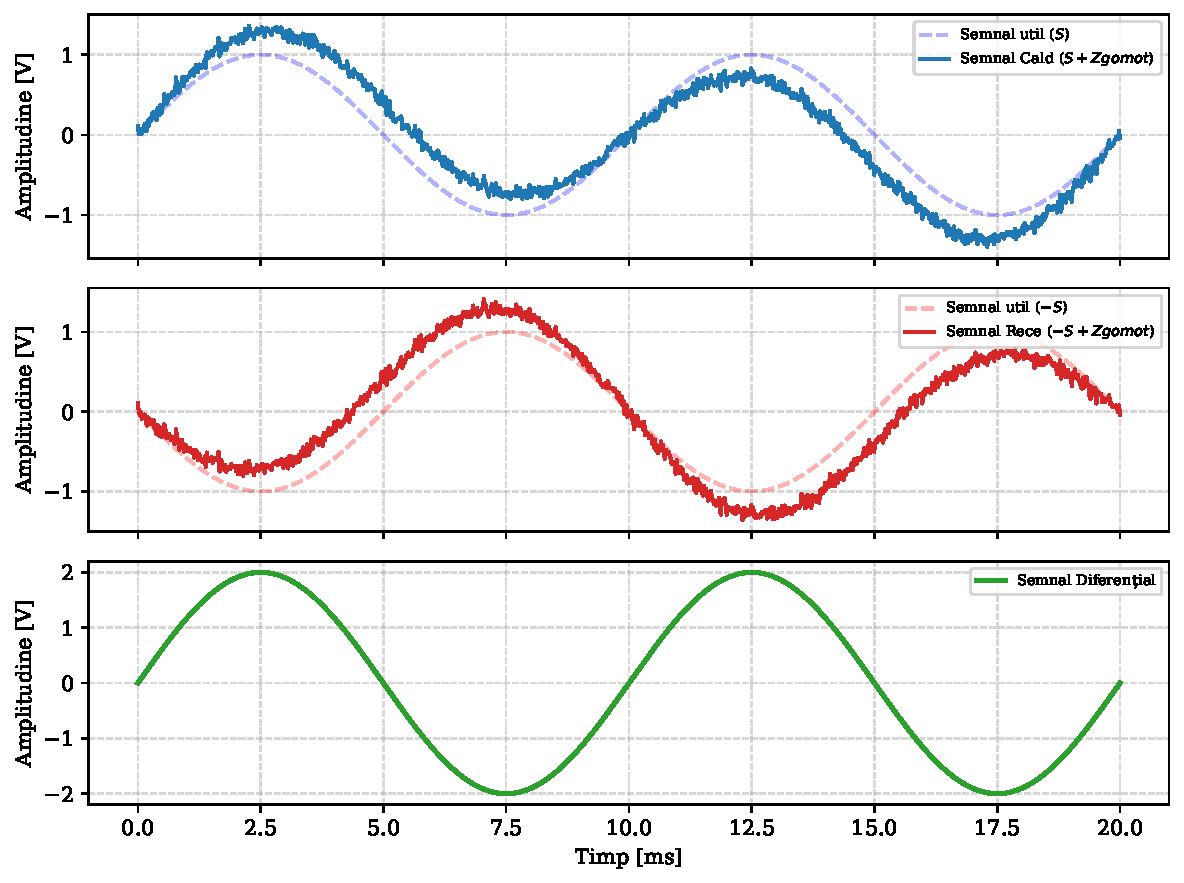
\includegraphics[width=0.7\textwidth]{figuri/cmrr_signals.pdf}
    \caption{Reprezentarea anulării zgomotului de mod comun prin transmisie echilibrată}
    \label{fig:cmrr_signals}
\end{figure}

Pentru a realiza această operație în domeniul analogic, se utilizează un amplificator diferențial, a cărui schemă de principiu este prezentată în Figura \ref{fig:diff_amp_theory}.

\begin{figure}[H]
    \centering
    \begin{circuitikz}[scale=1.2, transform shape]
        \draw (4,2) node[op amp] (opamp) {};
        \draw (0,2.5) node[left] {IN- (Rece)} to[R, l=$R_1$, o-] (opamp.-);
        \draw (0,1.5) node[left] {IN+ (Cald)} to[R, l=$R_3$, o-] (opamp.+);
        \draw (opamp.-) -- ++(0,1) coordinate(fb1) to[R, l=$R_2$] ++(2.4,0) coordinate(fb2) -- (opamp.out);
        \draw (opamp.+) to[R, l=$R_4$] ++(0,-1.5) node[ground] {};
        \draw (opamp.out) to[short, -o] ++(1,0) node[right] {$V_{out}$};
    \end{circuitikz}
    \caption{Schema teoretică a unui amplificator diferențial}
    \label{fig:diff_amp_theory}
\end{figure}

Tensiunea la ieșirea amplificatorului diferențial ($V_{out}$) rezultă din legea superpoziției și se calculează cu ecuația:
\begin{equation}
    V_{out} = V_{Cald} \cdot \left( \frac{R_4}{R_3 + R_4} \right) \cdot \left( 1 + \frac{R_2}{R_1} \right) - V_{Rece} \cdot \left( \frac{R_2}{R_1} \right)
\end{equation}

Pentru a asigura o anulare perfectă a semnalului de mod comun, este strict necesară respectarea următoarei condiții:
\begin{equation}
    \frac{R_1}{R_2} = \frac{R_3}{R_4}
\end{equation}
Dacă această condiție este îndeplinită, ecuația se simplifică, iar sistemul amplifică exclusiv diferența de potențial dintre cele două intrări:
\begin{equation}
    V_{out} = \frac{R_2}{R_1} \cdot (V_{Cald} - V_{Rece})
\end{equation}

\subsection{Calculul și măsurarea raportului de rejecție (CMRR)}
Capacitatea reală a circuitului de a respinge interferențele este cuantificată prin parametrul \textbf{CMRR} (Common Mode Rejection Ratio). Conform standardului IEC 60268-3 \cite{iec60268_3}, acesta se definește ca raportul logaritmic între câștigul diferențial ($A_d$) și câștigul de mod comun ($A_{cm}$):
\begin{equation}
    CMRR [dB] = 20 \log_{10} \left| \frac{A_d}{A_{cm}} \right|
\end{equation}

Unde câștigul de mod comun, $A_{cm}$, reprezintă raportul dintre variația tensiunii de ieșire și variația tensiunii aplicate simultan pe ambele intrări. Într-un sistem ideal, $A_{cm}$ ar trebui să fie egal cu zero, conducând la un CMRR infinit.

Metodologia de măsurare standardizată presupune parcurgerea următorilor pași, fundamentați pe recomandările IEC 60268-3 \cite{iec60268_3} și bunele practici de laborator descrise de Douglas Self \cite{douglasself}:
\begin{enumerate}
    \item \textbf{Determinarea câștigului diferențial ($A_d$):} Se aplică un semnal sinusoidal de test (tipic $1\text{ kHz}$) între bornele „Cald” și „Rece”. Tensiunea rezultată la ieșire ($V_{out,d}$) permite calcularea factorului de transfer diferențial: $A_d = V_{out,d} / V_{in,d}$.
    \item \textbf{Determinarea câștigului de mod comun ($A_{cm}$):} Cele două borne de intrare se conectează într-un punct comun (în scurtcircuit), asupra căruia se aplică un semnal de test de amplitudine ridicată raportat la masă. Tensiunea reziduală măsurată la ieșire ($V_{out,cm}$) permite determinarea câștigului de mod comun: $A_{cm} = V_{out,cm} / V_{in,cm}$.
\end{enumerate}

Performanța acestui indicator este dictată în mod direct de toleranța de fabricație a rezistențelor utilizate, fenomen modelat în Figura \ref{fig:cmrr_tolerance}.

\begin{figure}[H]
    \centering
    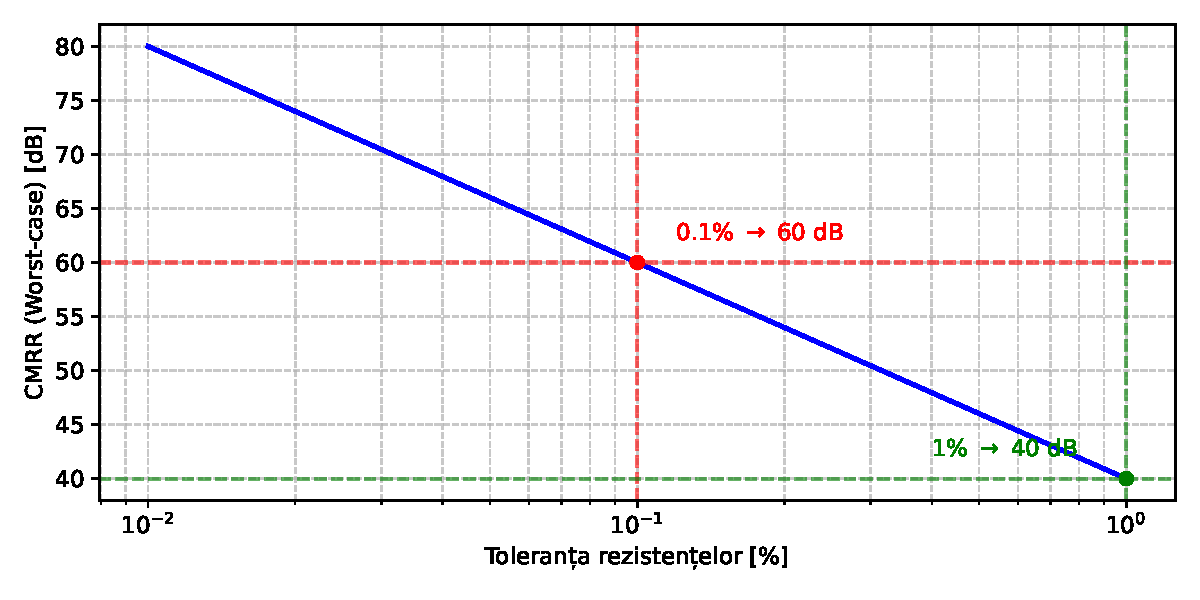
\includegraphics[width=0.8\textwidth]{figuri/cmrr_tolerance.pdf}
    \caption{Degradarea teoretică a parametrului CMRR în funcție de toleranța componentelor pasive}
    \label{fig:cmrr_tolerance}
\end{figure}

Pe baza analizei din Figura \ref{fig:cmrr_tolerance}, se observă că utilizarea unor rezistențe cu toleranță standard de $1\%$ plafonează valoarea CMRR la aproximativ $40\text{ dB}$, ceea ce este adesea insuficient pentru mediile electromagnetice zgomotoase. Obținerea unui nivel profesional de rejecție de minim $60\text{ dB}$ impune utilizarea exclusivă a componentelor pasive de precizie ridicată, cu o toleranță de maxim $0.1\%$ \cite{douglasself}.

\section{Procesarea digitală a semnalelor}
După condiționarea analogică, semnalul este digitizat prin procese de eșantionare și cuantizare, bazate pe teorema Nyquist-Shannon \cite{oppenheim2010discrete}.

\subsection{Eșantionarea și cuantizarea}
Conversia semnalului analogic în domeniu digital presupune două etape: eșantionarea (discretizarea în timp) și cuantizarea (discretizarea în amplitudine).

Conform teoremei Nyquist-Shannon \cite{oppenheim2010discrete}, pentru a evita fenomenul de \textbf{aliere spectrală} (aliasing) și a permite reconstrucția fidelă a semnalului, frecvența de eșantionare $f_s$ trebuie să fie cel puțin dublul frecvenței maxime din spectrul util ($f_s > 2 f_{max}$). În sistemele audio profesionale, se utilizează $f_s = 48\text{ kHz}$ sau chiar $f_s = 96\text{ kHz}$.

Cuantizarea presupune aproximarea amplitudinii fiecărui eșantion la cel mai apropiat nivel dintr-o scară definită pe $N$ biți, proces ilustrat în Figura \ref{fig:sampling}. Această aproximare introduce un \textbf{zgomot de cuantizare}, raportul semnal-zgomot ($SNR$) teoretic fiind determinat de numărul de biți de rezoluție conform relației fundamentale \cite{zolzer2011dafx}:

\begin{equation}
    SNR [dB] \approx 6.02 \cdot N + 1.76
    \label{eq:snr_quantization}
\end{equation}

În cazul sistemelor audio care utilizează o rezoluție de $N=24$ biți, raportul semnal-zgomot teoretic atinge valoarea de $146.24\text{ dB}$. Această performanță asigură o rezervă dinamică vastă, situând pragul zgomotului de cuantizare mult sub nivelul zgomotului componentelor analogice, eliminându-l astfel ca factor în lanțul de procesare.

\begin{figure}[H]
    \centering
    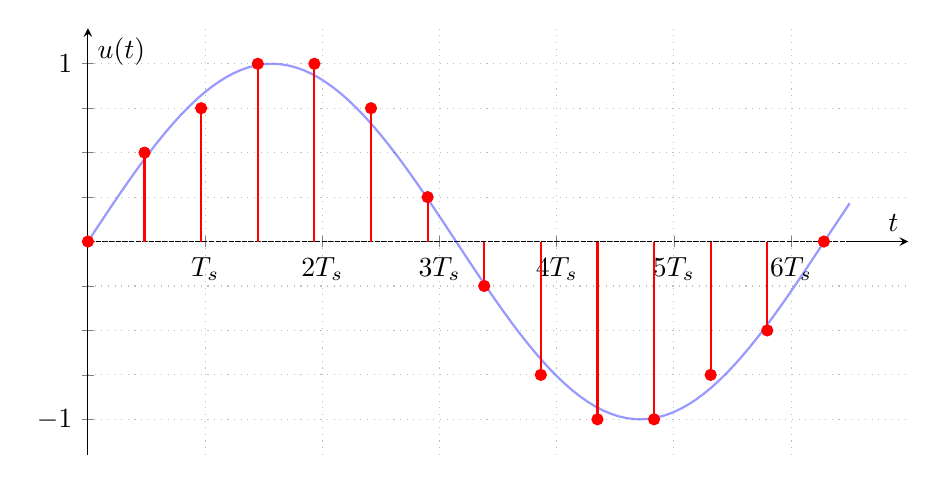
\begin{tikzpicture}
        \begin{axis}[
            axis lines = middle,
            xlabel = {$t$},
            ylabel = {$u(t)$},
            height=7cm, width=12cm,
            xmin=0, xmax=7,
            ymin=-1.2, ymax=1.2,
            xtick={0,1,2,3,4,5,6},
            xticklabels={0,$T_s$,$2T_s$,$3T_s$,$4T_s$,$5T_s$,$6T_s$},
            ytick={-1,-0.75,-0.5,-0.25,0,0.25,0.5,0.75,1},
            yticklabels={$-1$,,,,,,,,$1$}, 
            grid=both,
            grid style={dotted, gray!50}
        ]
            \foreach \y in {-1,-0.75,-0.5,-0.25,0,0.25,0.5,0.75,1} {
                \addplot [domain=0:6.5, gray!20, dotted, thin] {\y};
            }
            \addplot [domain=0:6.5, samples=100, blue, opacity=0.4, thick] {sin(deg(x))};
            \addplot [ycomb, red, thick, samples=14, domain=0:6.28] {round(sin(deg(x))*4)/4};
            \addplot [only marks, mark=*, red, samples=14, domain=0:6.28] {round(sin(deg(x))*4)/4};
        \end{axis}
    \end{tikzpicture}
    \caption{Procesul de eșantionare și cuantizare}
    \label{fig:sampling}
\end{figure}

\subsection{Convertoare Delta-Sigma ($\Delta\Sigma$)}
Conversia audio de înaltă rezoluție utilizează arhitecturi \textbf{Delta-Sigma} bazate pe supraeșantionare și modelarea zgomotului (noise shaping) \cite{zolzer2011dafx}. Prin operarea unui cuantizor de 1 bit la o frecvență mult peste pragul Nyquist, zgomotul de cuantizare este distribuit spectral, iar bucla de feedback a modulatorului îl „împinge” către frecvențele ultrasonice.

La ADC, acest proces este urmat de un filtru de decimare care elimină zgomotul de înaltă frecvență și livrează datele la rezoluția țintă (ex. 24 biți). Simetric, la DAC, semnalul este interpolat și trecut printr-un modulator digital, valoarea medie fiind extrasă de un filtru analogic de reconstrucție.

\section{Amplificarea în Clasa D}
Amplificatoarele în clasa D, cunoscute și sub denumirea de amplificatoare cu comutație, funcționează pe baza principiului modulării în lățime a impulsurilor (PWM). Spre deosebire de clasele de amplificare liniare, în care tranzistoarele de putere operează în regiunea activă, în clasa D acestea funcționează exclusiv ca întrerupătoare, fiind fie în stare de conducție (saturație), fie în stare de blocare \cite{self2006audio}.

Procesul de amplificare presupune transformarea semnalului audio analogic într-un semnal PWM. Această conversie se realizează prin compararea semnalului de intrare cu o undă purtătoare (triunghiulară sau dinte de fierăstrău) a cărei frecvență este mult superioară limitei superioare a benzii audio. Rezultatul este un flux de impulsuri a căror durată este proporțională cu amplitudinea instantanee a semnalului audio. Acest semnal PWM comandă etajul de putere, care comută tensiunea de alimentare pe sarcină prin intermediul unei configurații de tip punte H \cite{douglasself}.

Recuperarea informației audio din semnalul de putere modulat se realizează cu ajutorul unui filtru trece-jos pasiv de tip LC, plasat înainte de ieșire. Filtrul acționează ca un integrator, eliminând componentele de înaltă frecvență ale purtătoarei și lăsând să treacă doar valoarea medie a impulsurilor, care corespunde semnalului audio original. Această metodă de operare asigură transferul de putere către sarcină cu pierderi minime pe elementele active, deoarece tranzistoarele disipă putere semnificativă doar în timpul scurtelor tranziții între stările de conducție și blocare \cite{self2006audio}.

\chapter{Proiectarea Arhitecturii Hardware \label{hardware_design}}

În acest capitol este detaliată proiectarea modulelor componente ale amplificatorului audio multicanal, pornind de la condiționarea semnalelor de intrare și terminând cu etajele de putere și sistemul de management al alimentării. Arhitectura generală a sistemului a fost concepută pentru a asigura un raport semnal-zgomot optim și o versatilitate ridicată în utilizare.

\section{Interfața de intrare și preamplificarea}
Pentru a asigura o compatibilitate maximă cu standardele audio profesionale și de larg consum, interfața de intrare a fost proiectată pentru a accepta atât semnale echilibrate (balansate), cât și neechilibrate, conform principiilor de adaptare în tensiune.

\subsection{Etajul de intrare balansat și nebalansat}
Sistemul utilizează amplificatoare operaționale de înaltă performanță \textbf{OPA2134} \cite{opa2134}, selectate pentru distorsiunile armonice extrem de scăzute ($0.00008\%$). 
\begin{itemize}
    \item \textbf{Intrarea Balansată:} Utilizează o configurație de amplificator diferențial cu rezistențe de precizie de $10\text{ k}\Omega$ (R7, R8, R24, R25). Pentru a atinge un CMRR de peste $60\text{ dB}$, s-au utilizat componente cu o toleranță de $0.1\%$. Protecția împotriva interferențelor de radiofrecvență este asigurată de filtre trece-jos RC ($100\text{ }\Omega / 100\text{ pF}$) plasate la intrare.
    \item \textbf{Intrarea Nebalansată:} Utilizează un buffer cu impedanță ridicată, asigurând izolarea sursei de etajele ulterioare de procesare.
\end{itemize}

\subsection{Selectarea câștigului (+4 dBu / -10 dBV)}
Adaptarea nivelurilor de semnal este realizată printr-un etaj de amplificare cu câștig selectabil, comandat de comutatorul \textbf{SW1}. Acesta modifică configurația rețelei de feedback a preamplificatorului, utilizând un set de rezistențe calculate pentru a compensa diferența de nivel dintre standardele profesionale și consumer:
\begin{itemize}
    \item Pentru nivelul de $+4\text{ dBu}$ ($1.228\text{ V}_{rms}$), etajul funcționează cu un câștig apropiat de unitate sau o ușoară atenuare.
    \item Pentru nivelul de $-10\text{ dBV}$ ($0.316\text{ V}_{rms}$), se activează o treaptă de amplificare suplimentară utilizând rezistențe precum R12 ($8.2\text{ k}\Omega$) și R13 ($6.2\text{ k}\Omega$), aducând semnalul la valoarea nominală internă.
\end{itemize}

\section{Procesarea Digitală a Semnalului (DSP)}
Nucleul sistemului este procesorul \textbf{ADAU1701} \cite{adau1701}, care funcționează la o frecvență de eșantionare de $48\text{ kHz}$, sincronizat de un oscilator cu cristal de $12.288\text{ MHz}$.

\subsection{Condiționarea intrărilor ADC}
ADC-urile integrate în ADAU1701 necesită un semnal de intrare în curent. Pentru a converti tensiunea analogică în curent, s-au utilizat rezistențe serie de \textbf{$22\text{ k}\Omega$} (R33, R36 etc.). Această valoare, împreună cu condensatoarele de cuplaj de \textbf{$47\text{ }\mu\text{F}$}, stabilește o frecvență de tăiere inferioară de aproximativ $0.15\text{ Hz}$, asigurând un răspuns liniar în toată banda audio. Nivelul de intrare maxim (full-scale) este astfel setat la aproximativ $2\text{ V}_{rms}$, oferind un headroom suficient pentru procesare.

\section{Etajele de ieșire}
Sistemul dispune de două căi de ieșire independente pentru fiecare canal:
\begin{itemize}
    \item \textbf{Ieșiri de linie balansate:} Implementate cu drivere diferențiale, destinate interconectării cu alte echipamente profesionale.
    \item \textbf{Ieșiri de putere:} Utilizează module de amplificare în clasa D bazate pe circuitul integrat \textbf{TPA3118}. Acestea oferă o eficiență ridicată și sunt configurate pentru a conduce sarcini de $4\text{ }\Omega$ sau $8\text{ }\Omega$ la o tensiune de alimentare de $12\text{ V}$.
\end{itemize}

\section{Sistemul de alimentare și masa virtuală}
Alimentarea circuitelor analogice se realizează de la o sursă unipolară de $12\text{ V}$. Pentru a permite operarea amplificatoarelor operaționale în regim dual, s-a implementat un circuit de \textbf{masă virtuală} ($V_{cc}/2 = 6\text{ V}$).

Acesta este compus dintr-un divizor de tensiune rezistiv de înaltă impedanță ($100\text{ k}\Omega / 100\text{ k}\Omega$), bufferat de o secțiune a amplificatorului operațional \textbf{TL072}. Decuplarea masei virtuale se realizează cu condensatoare de $10\text{ }\mu\text{F}$, asigurând o referință stabilă și imună la zgomotul generat de etajele digitale și de putere.

\chapter{Implementarea Practică a Sistemului pe Perfboard \label{implementare}}
\section{Strategia de layout și asamblare}
Text în lucru...

\section{Realizarea modulelor individuale}
Text în lucru...

\section{Probleme întâmpinate la implementare}
Text în lucru...

\chapter{Testarea Sistemului și Analiza Performanțelor \label{testare}}
\section{Setup-ul de testare}
Text în lucru...

\section{Măsurători experimentale}
Text în lucru...

\section{Validarea funcționării programatorului și a algoritmilor DSP}
Text în lucru...

\section{Concluzii și direcții viitoare}
Text în lucru...


% --- BIBLIOGRAFIE ---
\bibliographystyle{unsrt}
\bibliography{referinte}

\end{document}
